\section{Overview of the proposed model}

The goal of our model is to estimate the 3D coordinates of all keypoints. First, we convert 2D depth images to 3D volumetric forms by reprojecting the points in the 3D space and discretizing the continuous space. After voxelizing the 2D depth image, the V2V-PoseNet takes the 3D voxelized data as an input and estimates the per-voxel likelihood for each keypoint. The position of the highest likelihood response for each keypoint is identified and warped to the real world coordinate, which becomes the final result of our model. Figure~\ref{fig:model_architecture} shows the overall architecture of the proposed V2V-PoseNet. We now describe the target object localization refinement strategy, the process of generating the input of the proposed model, V2V-PoseNet, and some related issues of the proposed approach in the following sections.

\begin{figure}[t]
\begin{center}
   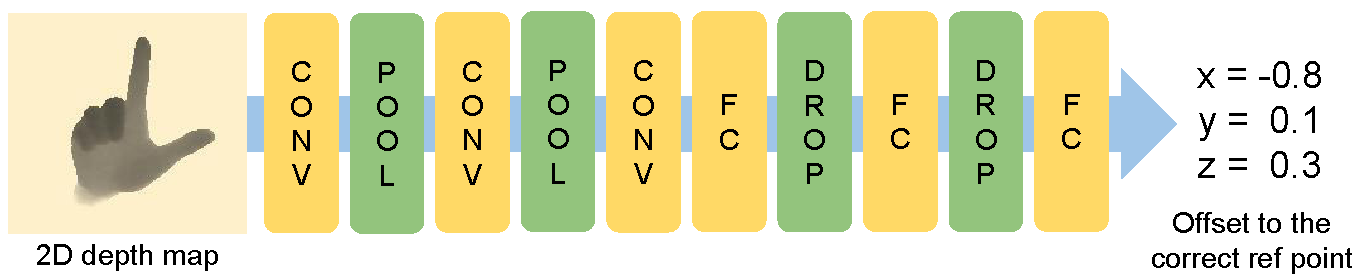
\includegraphics[width=1.0\linewidth]{ref_refine_net.pdf}
\end{center}
\vspace*{-5mm}
   \caption{Reference point refining network. This network takes cropped depth image and outputs the 3D offset from the current reference point to the center of ground-truth joint locations.}
\vspace*{-3mm}
\label{fig:ref_refine_net}
\end{figure}


